\chapter{Network simulation}

When evaluating the network performance of the implementations, we considered two options: using real IoT devices or using a network simulation tool.
Due to technical limitations that came with using real devices, such as not being able to access the router of our network, we opted for simulation.
In this chapter, we will discuss how we used Mininet~\citep{lantz_mininet_2021}, a realistic virtual network, in our evaluation.

Mininet is a tool that network developers and researchers can use to create software-defined networks (SNDs) using the $OpenFlow$ standard.

\begin{figure}[ht]
    \centering
    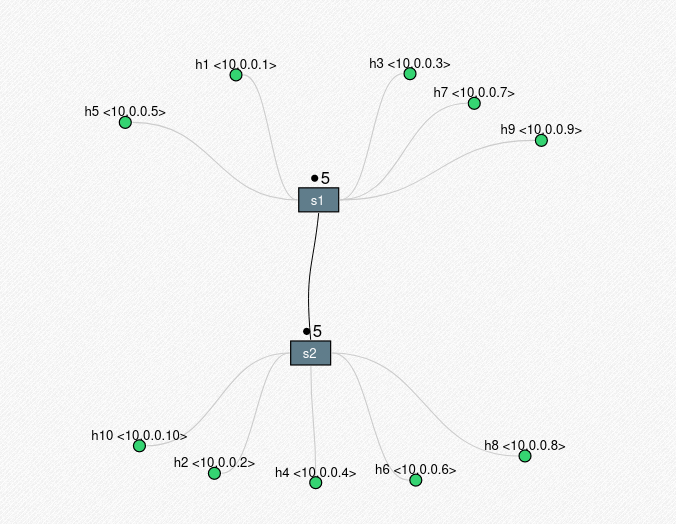
\includegraphics[width=0.5\linewidth]{images/mininet_topo.png}
    \caption{The resulting Dumbbell topology with 5 hosts on either side of the switch. This topology simulates congestion on the link as the hosts have to share it for their data transfer.}
    \label{fig:mininet-topo}
\end{figure}

Using the Python API provided, we created the network topology shown in Figure~\ref{fig:mininet-topo}.
The script takes several parameters to create a simulation environment resembling a realistic scenario.
The variables that the script changes between simulations are the link's \textit{bandwidth}, \textit{delay} and the rate of \textit{packet loss}.

The bandwidth of a link is the maximum rate of data transfer we can achieve.
In contrast to bandwidth in signal processing, we measure bandwidth in bits per second rather than hertz in computer networking.
The delay of a link specifies the latency of the link.
It is the time that a bit of data has to travel across a link. 
We measure this in milliseconds.
Link delay corresponds to the geographical distance between the communicating parties; however, in the case of IoT, we can expect devices to be in local proximity.
Lastly, the packet loss rate shows the percentage of packets that were corrupted or dropped in transit.
Various protocols having to retransmit packets also adds to the delay of data transfer.
Importantly, we have only considered the typical circumstances of packet loss and have not included scenarios such as interference or packet loss attacks.

The bandwidth and delay numbers correspond, as closely as possible, to various link types in a network.
To do so, we have gathered data from the~\cite{ofcom_uk_2021} report on UK broadband speeds.
There were specific cases in which it was not possible to find this data in the report; hence it was augmented using a similar methodology in the work conducted by~\cite{previdi_is-is_2019} and in the case of ZigBee, the work by~\citet{alena_fault_2011}.

\begin{table}[ht]
    \caption{The parameters chosen for each link simulation in Mininet. The types of links were chosen as the most commonly occurring ones in IoT use cases. The data also assumes a typical IoT setup where most devices are within local geographical proximity. That is, the devices are communicating between each other within the range of one factory or site, with only the central node communicating with some server.}\label{tab:links}
    %\tt 
    \rowcolors{2}{}{gray!3}
    \begin{tabular}{@{}llll@{}}
        \toprule
        \textbf{Simulated Link Type} & \textbf{Link bandwidth (Mb/s)} & \textbf{Link delay (ms)} & \textbf{Packet loss rate (\%)} \\
        Wi-Fi                        & \texttt{30}                    & \texttt{10}              & \texttt{2}                     \\
        ZigBee                       & \texttt{0.25}                  & \texttt{5}               & \texttt{1}                     \\
        4G                           & \texttt{4}                     & \texttt{20}              & \texttt{1.5}                   \\
        3G                           & \texttt{1}                     & \texttt{40}              & \texttt{1.5}                   \\
        100Mb Ethernet               & \texttt{100}                   & \texttt{1}               & \texttt{0.2}                   \\
        \bottomrule
    \end{tabular}
\end{table}

It was complicated to find exact estimates for packet loss rates, with most sources describing approximations for a stable connection~\citep{sdu_ictp-sdu_2013} and not precise measurements.
Hence, the data are best estimates, cross-validated through the different sources and are not exact values.

Using the different links, we then transferred a file of equal size using the various QUIC implementations described in Chapter~\ref{chap:quic_impl} for the evaluation of QUIC implementations.

We evaluated the MQTT/QUIC implementation performance using the same topology and simulation parameters.
In general, MQTT allows for messages with a maximum size of approximately 260MB.
However, this is a huge message, and most publicly deployed brokers will reject it, so a general use-case was simulated.

Each topic in MQTT consists of a hierarchy of topic levels separated by a forward slash.
For example, in a smart home scenario, we may have a topic like $home/groundfloor/kitchen/temp$ to control the temperature in the kitchen via a smart thermostat.
A topic may also include a wildcard.
The topic string $home/groundfloor/+/temp$ includes a \textit{single-level} wildcard that will match an arbitrary string.
This would match the topic $home/groundfloor/lounge/temp$, but not match the topic $home/secondfloor/kitchen/temp$.
If a client wishes to subscribe to multiple topics with the same prefix, a \textit{multi-level} wildcard may be used.
For example, the topic $home/secondfloor/kitchen/\#$ can be used to subscribe to all topics with a prefix matching the string before the hash character.
Notably, brokers reserve topics for system messages starting with the \$ character.

Taking this into account, we opted for a smart home scenario to simulate the MQTT communication.
The data transmitted can be found in Appendix~\ref{appendix:mqtt_message}.